\documentclass[11pt]{article}
% ==== riverrun whitepaper — shared preamble (design level: Slippay) ====
\usepackage[T1]{fontenc}
\usepackage[utf8]{inputenc}
\usepackage[letterpaper,margin=1in,headheight=15pt]{geometry}
\usepackage{amsmath}
\usepackage{newpxtext}
\usepackage{newpxmath}
\let\Bbbk\relax
\usepackage{amssymb}
\let\openbox\relax
\usepackage{amsthm}
\usepackage[scaled=0.85]{beramono}
\usepackage{microtype}
\usepackage{xcolor}
\usepackage{graphicx}
\usepackage{booktabs}
\usepackage{array}
\usepackage{tabularx}
\usepackage{enumitem}
\usepackage{titlesec}
\usepackage{fancyhdr}
\usepackage{listings}
\usepackage[most]{tcolorbox}
\usepackage{tikz}
\usetikzlibrary{arrows.meta,positioning,calc,backgrounds}
\usepackage{seqsplit}
\usepackage[hidelinks]{hyperref}

% ---- riverrun palette: river teal + desert gold ----
\definecolor{river}{HTML}{0E4D64}   % deep teal — the accent (sections, links)
\definecolor{riversoft}{HTML}{2C6B80}
\definecolor{ink}{HTML}{14181F}
\definecolor{steel}{HTML}{5B6270}
\definecolor{rule}{HTML}{C9CDD6}
\definecolor{paper}{HTML}{FBFAF7}
\definecolor{gold}{HTML}{9A6B00}    % desert gold — measured / on-chain artifacts
\definecolor{codebg}{HTML}{F4F5F8}
\definecolor{good}{HTML}{1E7A46}
\definecolor{soft}{HTML}{EAF1F3}    % pale teal for intuition boxes

\hypersetup{colorlinks=true,linkcolor=river,urlcolor=river,citecolor=river}

% ---- section styling ----
\titleformat{\section}{\normalfont\Large\bfseries\color{river}}{\thesection}{0.7em}{}
\titleformat{\subsection}{\normalfont\large\bfseries\color{ink}}{\thesubsection}{0.6em}{}
\titlespacing*{\section}{0pt}{1.5\baselineskip}{0.5\baselineskip}

% ---- header/footer ----
\pagestyle{fancy}\fancyhf{}
\renewcommand{\headrulewidth}{0.4pt}
\renewcommand{\footrulewidth}{0pt}
\fancyhead[L]{\footnotesize\color{steel}\textsc{riverrun}}
\fancyhead[R]{\footnotesize\color{steel}The Anonymity Layer for Solana, Post-Quantum}
\fancyfoot[C]{\footnotesize\color{steel}\thepage}

% ---- theorem-like environments ----
\newtheoremstyle{riv}{0.8em}{0.8em}{}{}{\bfseries\color{river}}{.}{0.5em}{}
\theoremstyle{riv}
\newtheorem{claimx}{Claim}[section]
\newtheorem{property}{Property}[section]

% ---- Feynman intuition box (pale teal) ----
\newtcolorbox{intuition}{
  enhanced,breakable,colback=soft,colframe=river,boxrule=0pt,
  leftrule=2.5pt,arc=1pt,left=8pt,right=8pt,top=6pt,bottom=6pt,
  fonttitle=\bfseries\footnotesize\color{river},title={THE IDEA, PLAINLY}
}
% ---- measured / on-chain artifact box (gold) ----
\newtcolorbox{measured}[1][]{
  enhanced,breakable,colback=paper,colframe=gold,boxrule=0pt,
  leftrule=2.5pt,arc=1pt,left=8pt,right=8pt,top=6pt,bottom=6pt,
  fonttitle=\bfseries\footnotesize\color{gold},title={\MakeUppercase{Measured}\ #1}
}
% ---- honest-limit box (steel) ----
\newtcolorbox{honest}{
  enhanced,breakable,colback=codebg,colframe=steel,boxrule=0pt,
  leftrule=2.5pt,arc=1pt,left=8pt,right=8pt,top=6pt,bottom=6pt,
  fonttitle=\bfseries\footnotesize\color{steel},title={WHAT THIS IS NOT}
}

% ---- code listing style ----
\lstset{
  basicstyle=\ttfamily\footnotesize,
  backgroundcolor=\color{codebg},
  frame=single,framesep=6pt,rulecolor=\color{rule},
  breaklines=true,columns=fullflexible,keepspaces=true,
  showstringspaces=false,commentstyle=\color{steel}\itshape,
  xleftmargin=4pt,xrightmargin=4pt,aboveskip=1em,belowskip=1em,
}

% ---- helpers ----
\newcommand{\rescue}{\mathrm{Rescue}}
\newcommand{\keff}{k_{\mathrm{eff}}}
\newcommand{\code}[1]{{\ttfamily #1}}
\newcommand{\river}{\textsc{riverrun}}
\setlist{itemsep=2pt,topsep=3pt,parsep=0pt}
\renewcommand{\arraystretch}{1.15}
\setlength{\parskip}{0.45em}
\setlength{\parindent}{0pt}


\begin{document}

% ===================== TITLE =====================
\thispagestyle{empty}
\begin{center}
{\color{river}\rule{\textwidth}{1.2pt}}\\[1.5em]
{\Huge\bfseries riverrun}\\[0.6em]
{\LARGE\bfseries Behavioral Privacy on Solana, Measured}\\[0.8em]
{\large Hiding \emph{who} acted --- and a ruler for what that hiding is\\[0.2em] actually worth}\\[1.3em]
{\color{river}\rule{\textwidth}{0.6pt}}\\[1.0em]
\end{center}

\begin{center}
\begin{minipage}{0.80\textwidth}
\centering\itshape\color{ink}
riverrun, past Eve and Adam's, from swerve of shore to bend of bay,\\
brings us by a commodius vicus of recirculation.\\[0.2em]
\normalfont\footnotesize\color{steel} --- James Joyce, \emph{Finnegans Wake}, first line
\end{minipage}
\end{center}
\vspace{1.2em}

\begin{center}
\begin{minipage}{0.88\textwidth}
\small
\textbf{\itshape Abstract.} \itshape On a public ledger, hiding \emph{who} performed an
action is a different problem from hiding \emph{how much} money moved, and a harder
one to reason about honestly. This paper describes \river, a system for behavioral
privacy on Solana. A member commits an intent and later executes exactly that
intent, while no observer can say which member did it. The proof is a transparent,
post-quantum STARK that welds membership, a per-round nullifier, and the public
action into one object, with no trusted setup; a synchronized round of $k$ members
collapses into a single proof and a single verification. The paper's second half is
a warning aimed at \river\ and at every system like it. Every anonymity pool
advertises a number, $1/k$, that counts members --- and that number is a fiction,
because it ignores where the members' money came from, and the funding graph is
public. We give a ruler, the effective anonymity-set size of Serjantov and Danezis
conditioned on funding provenance, and run it against a live pool on Solana
mainnet: a set advertising $k=30$ delivers an effective $6.5$, and one member has an
anonymity of exactly one. Because \river\ can \emph{measure} a crowd's anonymity, an
agent can \emph{form} a good one on purpose --- and hand each member a
proof-carrying certificate they verify without trusting the agent. Every claim of
the form ``$X$ is bound'' has a test verified to fail without the constraint it
tests; three such tests turned out to be decorative, and we say which. Where the
system does not yet hold --- an unaudited circuit, off-chain verification,
example-grade parameters --- we say so plainly. Every number here is reproducible
from one command.
\end{minipage}
\end{center}
\vspace{1.0em}

\begin{center}
\small\color{steel}
Manuel Guilherme Galmanus \quad\textbullet\quad Independent Researcher \quad\textbullet\quad Preprint, July 2026
\end{center}

\vspace{0.5em}
{\color{rule}\hrule}
\vspace{0.3em}
{\small\tableofcontents}
\vspace{0.3em}
{\color{rule}\hrule}
\clearpage

% ===================== 1. INTRODUCTION =====================
\section{The problem, in one picture}

Imagine a town where every letter anyone ever mailed is pinned to a public board,
forever. Not the contents --- those are sealed --- but the envelopes: who sent what
to whom, when, and how heavy the package was. You would learn a great deal about
that town without opening a single letter. Who pays whom. Who is suddenly buying.
Who moves money at three in the morning. Who copies whose move an hour later.

A public blockchain is that board. People imagine that a wallet address, being a
random string and not a name, keeps them private. The opposite is closer to the
truth. The address is a stable handle, and everything done under it accumulates
into a pattern --- a \emph{behavioral fingerprint}. When you act, how much, which
protocols you touch, in what order: that is enough for modern chain-analysis to
cluster your wallets, attach an identity, and increasingly to predict and front-run
what you will do next. The tools that do this improve every month, because the data
is permanent and public and the models feeding on it are hungry.

The dominant view of on-chain privacy assumes the problem is the money: hide the
amounts, hide the balances. \emph{This view is incomplete.} There are two kinds of
privacy here and they are not the same. One hides \emph{how much}. The other hides
\emph{who} --- which person, out of a crowd, performed a public action. Most work
has gone into the first: confidential transfers, shielded balances, mixers that
break the link between a deposit and a withdrawal of value. This paper is about the
second. Amounts are not hidden here and are not the point. What we sever is the link
between an \emph{actor} and an \emph{action}.

\begin{intuition}
Richard Feynman said that if you cannot explain a thing simply, you do not
understand it. So here is the whole idea in one sentence, and the rest of the paper
is only this sentence made precise and made real: \textbf{you disappear into a crowd
of people who all look like they could have done the thing you did.}
\end{intuition}

\begin{intuition}
\textbf{On the name.} \emph{Finnegans Wake} (James Joyce, 1939) is a novel with no
beginning. Its last sentence breaks off mid-phrase --- ``a way a lone a last a
loved a long the'' --- and runs straight into its first word, ``riverrun.'' The
book is a circle. It is written in a dream-language where every word carries many
meanings at once, and it runs on Giambattista Vico's theory that history moves in
cycles that return to their start; the pun ``a commodius vicus of recirculation''
hides Vico's name. Its river, Anna Livia, flows to the sea and comes back as rain.
We did not choose the name for the poetry. Three of the book's ideas turn out to
be load-bearing, and each is cashed out as a number or a construction later:
\begin{itemize}[leftmargin=1.2em,itemsep=0.1em,topsep=0.2em]
\item \textbf{A circle has no beginning.} The book's core structural fact --- no
origin, no source --- is exactly the defense against the funding-graph attack of
Section~\ref{sec:ruler}: a funding trail that loops has no origin to trace.
\item \textbf{The \emph{ricorso}}, Vico's return that begins the cycle again, is
how the anonymity set is reborn each cycle so history stops accumulating
(Section~\ref{sec:ricorso}).
\item \textbf{Irreducible polysemy.} Every word in the book has many valid
meanings at once, none privileged; ``which is the real one'' is a category error,
not a puzzle. This is the ambiguous-origin construction of
Section~\ref{sec:ruler}, where the funding trail reaches many origins with none
privileged, so which is real is \emph{undefined} rather than hidden --- measured
at $2.90$ bits of doubt.
\item \textbf{``Here Comes Everybody.''} The protagonist HCE is at once one man
and everyone --- an identity dissolved into the crowd, which is what an anonymity
set is. \emph{Disanalogy:} HCE is a single dream-figure who is everyone, whereas
here there are many real members and the cryptography makes which one acted
genuinely undefined, not merely hard to guess.
\end{itemize}
\end{intuition}

\subsection{Contributions}

\begin{enumerate}[leftmargin=1.5em]
\item \textbf{A behavioral-privacy pool} whose proof welds membership, a per-round
      nullifier, and the public action into one transparent, post-quantum STARK,
      with no trusted setup (Sections~\ref{sec:idea}--\ref{sec:round}).
\item \textbf{The ricorso}: a rebirth of the anonymity set each cycle that closes a
      cross-epoch linkage leak the basic construction has (Section~\ref{sec:ricorso}).
\item \textbf{A ruler} --- the effective anonymity-set size conditioned on funding
      provenance --- run against a live mainnet pool, and turned into a user-facing
      pre-flight defense (Section~\ref{sec:ruler}).
\item \textbf{A coordinator}: an agent that uses the ruler \emph{generatively} to
      form rounds that maximize measured anonymity, and hands each member a
      proof-carrying certificate they verify without trusting it
      (Sections~\ref{sec:coord}--\ref{sec:axl}).
\item \textbf{Measured on-chain cost} for the whole thing, down to the compute unit,
      with an honest account of what fits and what does not
      (Section~\ref{sec:cost}).
\end{enumerate}

% ===================== 2. THE IDEA =====================
\section{The idea: commit an intent, execute it unlinkably}
\label{sec:idea}

Tornado Cash, the Ethereum mixer, breaks the link between putting money \emph{in}
and taking money \emph{out}. You deposit one coin; later, from a fresh address, you
withdraw one coin, proving in zero knowledge that you are owed a withdrawal without
revealing which deposit was yours. The pool is a crowd, and you hide in it.

\river\ keeps the shape and changes the payload. Instead of a coin, the hidden thing
is a \emph{behavior}. Three steps.

\textbf{Commit.} A member publishes $\ell = \rescue(s, a)$ into a public set, where
$s$ is a secret only they know and $a$ is the action they intend --- ``swap $1$ SOL
for USDC on venue V'', encoded as a hash. Publishing $\ell$ announces that
\emph{somebody in this set intends action $a$}, revealing nothing about who. The set
is a Merkle tree; its root $R$ is the public fingerprint of the crowd.

\textbf{Execute.} Later --- ideally in a synchronized round where many members do the
same thing at once --- the member performs $a$ from a fresh identity with a
zero-knowledge proof of one sentence: \emph{``I know a secret $s$ whose commitment
$\rescue(s,a)$ is a leaf under the public root $R$, and my nullifier this round is
$n = \rescue(s, r)$.''} The action is public. The author is not.

\textbf{Settle.} The pool verifies the proof, checks the nullifier $n$ is fresh this
round, spends it, and releases the action. The public transcript is $\{R, a, n\}$,
with no link to any commitment.

Two questions decide whether this is privacy or theater, and both concern the
nullifier. Why have one? Because without it a member could act a thousand times from
a thousand fresh identities, and the ``crowd'' would be one person in a thousand
masks. The nullifier is a token derived from the secret and the round, spendable
once per round. It reveals nothing about $s$, and the nullifiers one member produces
in different rounds cannot be tied together. So it enforces ``one action per member
per round'' while never naming the member. This is a studied primitive; PLUME
\cite{plume} formalizes exactly this and proves its uniqueness and secrecy.

The subtle question: how does anyone know the revealed $n$ came from the \emph{same}
secret that proved membership? If those two facts are proven separately, a member
could prove membership honestly and then present a stranger's nullifier --- spending
someone else's turn, or hiding that they spent their own. The two halves must be
welded inside one proof. Getting that weld right, and \emph{knowing} it is right, is
the heart of the next section.

% ===================== 3. THE PROOF =====================
\section{The proof: one object, three bindings}
\label{sec:proof}

A zero-knowledge proof convinces you a statement is true while revealing nothing
beyond its truth. Two families are used on blockchains, and the choice is a real
fork with real costs on each side.

Pairing-based SNARKs (Groth16) give tiny proofs --- a couple of hundred bytes --- that
verify cheaply. Their price is a \emph{trusted setup}: a one-time ceremony must
generate a structured proving key, and if that ceremony's secret randomness is ever
recovered, the system can be forged. For a Merkle circuit the key is tens of
megabytes that must be produced, trusted, and shipped to every prover. And the
security rests on elliptic curves, which a large quantum computer breaks.

STARKs are built from a hash function alone. No pairings, no ceremony, no per-circuit
setup; security rests on hash collision-resistance, believed to survive a quantum
adversary. The price is proof size: kilobytes, not bytes. \river\ takes this side,
deliberately, and Section~\ref{sec:cost} measures exactly what it costs and buys.

\begin{intuition}
\textbf{What a STARK is, in one paragraph.} Write your computation as a big table:
rows are time-steps, columns are registers, arranged so ``it was computed
correctly'' becomes ``every adjacent pair of rows obeys a fixed rule.'' Turn each
column into a polynomial through its values. The rules become equations those
polynomials must satisfy. The prover commits to the polynomials and the verifier
challenges them at random points; a cheat would need a \emph{wrong} low-degree
polynomial to agree with a right one almost everywhere, which is impossible unless
they are equal. FRI is the machinery that lets the verifier confirm ``this really is
low-degree'' by folding it in half over and over and spot-checking. The disanalogy
with a normal exam: the verifier never sees the answers, only a few random cells and
a proof that all the cells are consistent --- which is why the witness stays hidden.
\end{intuition}

\subsection{What the circuit proves}

\river\ uses a STARK over a Rescue-Prime \cite{rescueprime} Merkle tree --- an
arithmetization-oriented hash chosen because it is cheap to express as polynomial
constraints. The proof's public inputs are the four-tuple $\{R,\,n,\,r,\,a\}$: root,
nullifier, round, action. Its private inputs --- the witness --- are the secret $s$,
the leaf's position, and the Merkle path. One secret must satisfy all three at once:

\begin{enumerate}[leftmargin=1.5em,itemsep=0.1em]
\item \textbf{Membership.} $\rescue(s, a)$ is a leaf under $R$, via the private path.
\item \textbf{Nullifier binding.} $n = \rescue(s, r)$: the revealed nullifier is
      this member's, this round.
\item \textbf{Action binding.} The leaf that resolves to $R$ commits to the public
      action $a$: the member executes the intent they registered, not another.
\end{enumerate}

Because all three read the same private $s$, no member can mix and match. That is the
weld.

\begin{figure}[h]
\centering\small
\begin{tabular}{@{}c|cccccc|c|cc@{}}
\toprule
col & \multicolumn{6}{c|}{Rescue state $0\dots5$} & bit $6$ & \multicolumn{2}{c}{carry $7,8$}\\
\midrule
cycle 0 & \multicolumn{6}{c|}{hash $(s_0,s_1,r)\to$ nullifier $n$} & --- & $s_0$ & $s_1$\\
row 7 (load) & \multicolumn{2}{c}{$s_0,s_1$} & \multicolumn{2}{c}{$a_0,a_1$} & \multicolumn{2}{c|}{$0$} & --- & \multicolumn{2}{c}{cleared}\\
cycles $1..d{+}1$ & \multicolumn{6}{c|}{Merkle path up to root $R$} & path bit & \multicolumn{2}{c}{---}\\
\bottomrule
\end{tabular}
\caption{The width-9 trace. Cycle 0 computes the nullifier; row 7 loads the leaf
preimage --- the same secret plus the public action --- so the leaf commits to both;
the rest walks the path to $R$. A single constraint at row 0, the ``start-tie'',
forces the nullifier's input to equal the carried secret. The carry is confined to
cycle 0 on purpose (Section~\ref{sub:leak}).}
\label{fig:trace}
\end{figure}

\subsection{Knowing the weld holds}

A privacy proof that is subtly wrong is worse than no proof: it advertises a
guarantee it does not deliver. So the interesting question is not ``did we write the
constraints'' but ``do they bite.'' The method used throughout \river\ is
\emph{mutation testing}: for every claim ``$X$ is bound'' there is a test, and we
delete the constraint meant to enforce $X$ and confirm the test then fails. If
deleting it changes nothing, the test was passing for some other reason and is
worthless.

This is not a formality. Three tests written during development were exactly that
worthless, and mutation testing is how they were caught.

\begin{itemize}[leftmargin=1.4em,itemsep=0.15em]
\item The action-binding tests checked that announcing a different public action was
      rejected. They passed even with the binding deleted --- the action feeds the
      Fiat--Shamir transcript, so a mismatched public input is rejected anyway, for a
      reason unrelated to the constraint. The real attack, which the useful test
      performs, hashes the committed action into the leaf (so the path still
      resolves) while \emph{announcing} a different one. Delete the constraint and
      that forged proof verifies.
\item The nullifier tests that only varied public inputs passed on boundary
      assertions alone, with no start-tie. The test that guards the weld builds the
      attacker's trace: hash secret $A$, carry member $B$ into the path.
\item In the ricorso a whole check --- that the migration nullifier comes from the
      migrating secret --- had \emph{no} test until a mutation left everything green.
\end{itemize}

\begin{honest}
None of this makes the circuit audited. It is hand-rolled, and a passing negative
test is necessary, not sufficient, for soundness. An independent review is named on
the roadmap, not glossed over. What mutation testing removes is a specific, common,
embarrassing failure: tests that look like they prove something and prove nothing.
\end{honest}

\subsection{A leak we found by measuring}
\label{sub:leak}

The first version of the circuit carried the secret in two columns held
\emph{constant} across the whole trace. This looked harmless. It was not. A STARK
opens the prover's committed data at random points, and a constant column has a
constant low-degree extension --- so the secret appeared, verbatim, in essentially
every opening. We knew only because a test checked, over many proofs, whether the
raw secret bytes appeared in the proof. They did: twenty times out of twenty.
Confining the carry to the eight rows where it is needed fixed it: zero out of
twenty. A single-sample test would have missed it. This is why we say ``the witness
is not on the wire'' and \emph{not} ``zero-knowledge'': the underlying prover does
not randomize the witness, so formal zero-knowledge is a claim we decline to make.

% ===================== 4. THE ROUND =====================
\section{The synchronized round: one crowd, one proof}
\label{sec:round}

The privacy argument rests on a crowd. If $k$ members do the same action in the same
round, an observer's chance of attributing any one execution is at best $1/k$. The
natural way to run this is a synchronized round: many members acting identically at
one moment, so there is no timing and no ordering to separate them.

A small observation with a large payoff: that synchronized round is exactly the
structure that lets many proofs collapse into one. A STARK is a statement about an
execution trace. The $k$ members' sub-traces are independent, so they lay end to end
into one longer trace, the per-cycle constraints repeating along it, with a
\emph{seam} that switches off the linking logic at each boundary so one member's last
row does not bleed into the next member's first. One proof for the whole round, and
one verification.

\begin{measured}[--- batching a synchronized round]
\centering
\begin{tabular}{rrrr}
\toprule
members $k$ & one batched proof & $k$ separate proofs & saving \\
\midrule
$4$  & $19{,}772$ B & $45{,}300$ B     & $2.3\times$ \\
$64$ & $43{,}684$ B & $1{,}074{,}169$ B & $24.6\times$ \\
\bottomrule
\end{tabular}\\[0.3em]
{\footnotesize At $k{=}64$ a per-member scheme ships over a megabyte of proof and
needs $64$ verifications; the batched round is one proof, one verification.}
\end{measured}

\begin{honest}
Two structural limits. The prover of a batched round must know every member's
secret. For a crowd of distrustful strangers that is a custodian, not privacy, and
would need distributed proving. But for one operator running $k$ identities --- an
agent fleet, a market maker --- one prover holds all $k$ secrets already, and the
$24.6\times$ is real. And batching trades prover time for proof size: the trace is
$k$ times longer and proving is super-linear, so the round costs more wall-clock than
the sum of individual proofs. It is the right trade when the scarce resource is
on-chain verifications.
\end{honest}

% ===================== 5. THE RICORSO =====================
\section{The ricorso: the crowd is reborn}
\label{sec:ricorso}

Now the name earns its keep. \emph{Finnegans Wake} runs on Vico's cycle of history:
ages that repeat, and a fourth age, the \emph{ricorso}, the return that begins it
again. \river\ borrows the book's circularity twice --- here, and for the funding
graph in Section~\ref{sec:ruler}.

The leak the ricorso closes is easy to miss. A member's per-round nullifier changes
every round, unlinking one execution from another. But their \emph{leaf},
$\rescue(s,a)$, never changes: published once at commit, it stays forever. Two
consequences. Anyone who ever learns your leaf --- a bug, a subpoena, a careless
client --- links you across every round you ever acted in; the nullifiers protect
executions from each other, but nothing protects a member from their own history.
And a set that only grows is a public record: join-order is a timeline of who
arrived when.

The ricorso lets the set be reborn each cycle. A member holds a fresh secret per
cycle, $s_c = \rescue(s, c, \textsf{dom}_{\text{cycle}})$, and a fresh leaf $\ell_c =
\rescue(s_c, a)$, and at each rebirth proves the new leaf descends from \emph{some}
leaf under the previous root --- without revealing which. A migration nullifier,
spent once per cycle, stops one seat from becoming several. The two domain tags must
differ, or publishing a migration nullifier would leak the next cycle's secret; the
implementation pins that with a test. History stops accumulating.

\begin{honest}
The relation is implemented and mutation-tested \emph{in the clear}; the STARK that
proves it without the witness is specified, not built. The reason is concrete: the
migration circuit needs five hash cycles before the path, which shifts valid
set sizes to $\{8, 2048\}$ while the execution circuit needs $\{4, 64, 16384\}$, and
the two do not intersect. Shipping it means realigning both --- a day on the most
delicate code, and the honest place to stop, with the execution path green, is at
the specification. It is exactly where the nullifier binding stopped before it was
later built and mutation-verified.
\end{honest}

% ===================== 6. THE RULER =====================
\section{The ruler: your $k$ is not your $k$}
\label{sec:ruler}

Everything so far builds the pool. This section measures it, and applies not only to
\river\ but to every anonymity pool of this kind. It is, we think, the most useful
part of the paper, because it names a number that is quietly wrong across a whole
category of systems.

\subsection{The advertised number counts the wrong thing}

Every pool reports its privacy as $1/k$: $k$ members, so a one-in-$k$ guess. That
counts \emph{members}, and assumes they are interchangeable. They are not, because of
where their money came from. Every member funded their wallet somehow, and the
funding trail is public. Trace it backward and you often reach an attributable
origin: an exchange's withdrawal address, a known service, a doxxed funder. Sort the
set by these origins. If the acting identity's origin is observable too --- and a
fresh withdrawal wallet must be funded from \emph{somewhere} --- then learning it
does not leave $k$ suspects. It leaves only the members who share that origin. The
crowd you are hidden in is your \emph{provenance class}, not the whole set.

\begin{intuition}
This is the same shape as the paper's opening claim about privacy in general: there
is a \emph{defended surface} everyone looks at (the advertised $k$) and a
\emph{larger real surface} behind it (the effective $k$, set by the funding graph).
Guarding the first while ignoring the second is the mistake, and here we can measure
exactly how big the gap is.
\end{intuition}

The measure itself is not new. Serjantov and Danezis \cite{serjantov2002} showed in
2002 that the honest quantity is not set size but the \emph{entropy} of the
distribution linking suspects to the event --- the effective anonymity-set size. And
measuring advertised-versus-true anonymity is an established programme on Ethereum
\cite{tutela,beres,crosschain,du}. Two things are new: the channel (funding
provenance, which those works do not condition on) and the chain (none of it has run
on Solana).

\subsection{The formula, and why its direction matters}

Partition the $k$ members into provenance classes of sizes $n_1, n_2, \dots$. The
adversary learns the actor's class $c$ with probability $n_c/k$, then guesses
uniformly among that class's $n_c$ members. The residual uncertainty is the average
over classes of the log of the class size:
\begin{equation}
H = \sum_c \frac{n_c}{k}\log_2 n_c, \qquad \keff = 2^{H}.
\label{eq:effk}
\end{equation}
$\keff$ is the size of the crowd the member is genuinely hidden in. One class holding
everyone gives $\log_2 k$: nothing was partitioned. All-singleton classes give
$H = 0$, an effective $k$ of one: every member identified.

\begin{intuition}
\textbf{Worked by hand.} Ten members: six funded from exchange A, three from B, one
alone. Advertised anonymity $1/10$. Condition on origin. With probability $6/10$ the
actor is an ``A'' and the adversary cannot tell which of six: $\log_2 6 \approx 2.58$
bits. With $3/10$, a ``B'': $\log_2 3 \approx 1.58$. With $1/10$, the lone member:
$0$ bits, identified. Average: $H = 0.6(2.58)+0.3(1.58)+0.1(0) = 2.02$ bits, so
$\keff \approx 4.1$. The pool sold ten and delivered four --- and the lone member has
an anonymity of exactly one, no matter how big the crowd behind them.
\end{intuition}

The \emph{direction} is the whole thing, and the first implementation had it
backwards. It is tempting to measure how \emph{concentrated} the classes are
(min-entropy of the distribution), but that reports catastrophe precisely when the
measurement found nothing to partition on: a single class of seven --- the happy case
--- came out as ``effective $k=1$'', when the honest reading is ``effective $k=7$.''
Following Serjantov and Danezis, and against the normalized variant that scores a set
of one as a perfect $1.0$, we use the residual entropy of Eq.~\ref{eq:effk} directly.
Four tests pin the direction; one caught the arithmetic a second time.

\subsection{The measurement}

We ran this against a live Tornado-style SOL privacy pool on Solana mainnet,
sampling $30$ real depositors and tracing each funding graph backward with a
bounded, public-RPC walk.

\begin{measured}[--- a live mainnet anonymity set]
\centering
\begin{tabular}{lr}
\toprule
depositors sampled & $30$ \\
reach an attributable origin & $11/30$ ($37\%$), mean $1.18$ hops \\
provenance classes & $12$ \\
\textbf{advertised $k$} & $\mathbf{30}$ \\
\textbf{effective $k$} & $\mathbf{6.5}$ \\
\textbf{worst case} & $\mathbf{1}$ \\
\bottomrule
\end{tabular}\\[0.3em]
{\footnotesize A set advertising $30$ delivers an effective $6.5$. One depositor sits
alone in their class: for them the pool provides no anonymity against an adversary
who reads the funding graph, while its dashboard reports one-in-thirty.}
\end{measured}

Three honesties. It is not a flaw in that pool: no deposit-pool design controls where
its users' money came from, which is exactly why the channel goes unmeasured and
keeps working. It is a \emph{floor}: a public RPC following only SOL to bounded depth
sees less than a funded analyst with a tag database, so the true leak is at least
this large. And $37\%$ sits in the same $20$--$35\%$ range that the Ethereum
literature \cite{crosschain} finds with behavioral heuristics on Tornado --- a sanity
check on the tool, not the pool.

\subsection{The same ruler, turned on \river\ --- and on the user}

Measuring others' pools and not your own is marketing. The same function runs over
\river's own constructions, against $2000$ synthetic members. There are three, and
they form a spectrum of increasing privacy that maps, exactly, onto three ideas
from the book (Figure~\ref{fig:cycle}):

\begin{center}\small
\begin{tabular}{lrrr}
\toprule
construction & reaches an origin & ``which origin'' & $\keff$ of $2000$ \\
\midrule
rooted decoy (the field) & $100\%$ & $0$ bits & $500$ \\
cyclic, \textbf{ambiguous} origin & $100\%$ & $\mathbf{2.90}$ bits & $2000$ \\
cyclic, \textbf{rootless} & $0\%$ & --- & $2000$ \\
\bottomrule
\end{tabular}
\end{center}

The first row is what the field ships: every trail ends at one attributable origin,
so there is no doubt about where the money came from, and the crowd collapses to
$500$. The third row is the \emph{circularity} insight --- a funding cycle with no
beginning, so there is no origin at all to trace, and the set is worth its full
$2000$.

The middle row is the fourth insight, and it is worth dwelling on because it is the
strongest one in practice. In \emph{Finnegans Wake}, a word does not hide its ``real''
meaning behind the others; it \emph{has} no single real meaning. Every reading is
valid, none is privileged, and asking which one Joyce intended is a category error
--- the ambiguity is the meaning. The \textbf{ambiguous-origin} construction is that
idea made numeric. The funding trail does reach origins --- $100\%$ of the time --- but
it reaches \emph{many}, arranged so that none is privileged, so ``which is the real
origin'' is not hidden, it is \emph{undefined}. We measure $2.90$ bits of residual
doubt about which, and the set stays worth its full $2000$.

Why this is the strongest in practice: rootlessness is an idealization. It holds
only while a construction's funding sources are \emph{themselves} unattributable,
and the moment one of them is a known exchange, the ``no origin'' claim fails. But it
does not fail to nothing --- it degrades exactly to \emph{ambiguity}: now there is a
reachable origin, but still no way to say it is \emph{the} one. Ambiguity is where
rootlessness lands when it meets the real world, and it is where the defense actually
lives.

\begin{honest}
The disanalogy, and the limit. The book's polysemy is inherent to language; here the
ambiguity is \emph{constructed} --- a funding graph deliberately built so that
multiple origins are symmetric, so no attribution can privilege one. And it defends a
specific thing: attribution to a \emph{particular} origin, not membership in the
\emph{group} of origins. If an adversary needs only ``this came from one of these
three exchanges'' rather than which, ambiguity does not stop them. It buys $2.90$ bits
of ``which'', not membership secrecy.
\end{honest}

\begin{figure}[h]
\centering
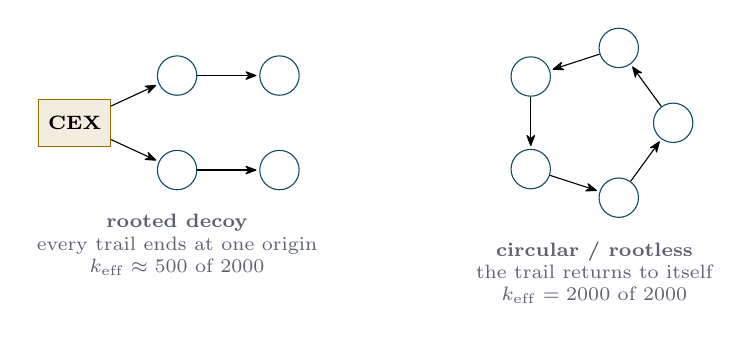
\begin{tikzpicture}[
  >={Stealth[round]}, node distance=13mm,
  w/.style={circle,draw=river,minimum size=5mm,inner sep=0pt,font=\scriptsize},
  hub/.style={rectangle,draw=gold,fill=gold!12,minimum size=6mm,font=\scriptsize\bfseries},
  every edge/.style={draw,->,shorten >=1pt}
]
\node[hub] (root) at (0,0) {CEX};
\node[w] (a1) at (1.3,0.6) {}; \node[w] (a2) at (2.6,0.6) {};
\node[w] (a3) at (1.3,-0.6) {}; \node[w] (a4) at (2.6,-0.6) {};
\draw (root) edge (a1); \draw (a1) edge (a2);
\draw (root) edge (a3); \draw (a3) edge (a4);
\node[font=\scriptsize,align=center,color=steel] at (1.3,-1.55) {\textbf{rooted decoy}\\ every trail ends at one origin\\ $\keff \approx 500$ of $2000$};
\begin{scope}[xshift=6.6cm]
\node[w] (c1) at (0:1) {}; \node[w] (c2) at (72:1) {}; \node[w] (c3) at (144:1) {};
\node[w] (c4) at (216:1) {}; \node[w] (c5) at (288:1) {};
\draw (c1) edge (c2); \draw (c2) edge (c3); \draw (c3) edge (c4);
\draw (c4) edge (c5); \draw (c5) edge (c1);
\node[font=\scriptsize,align=center,color=steel] at (0,-1.9) {\textbf{circular / rootless}\\ the trail returns to itself\\ $\keff = 2000$ of $2000$};
\end{scope}
\end{tikzpicture}
\caption{Two ways to fund a crowd. Left: every wallet traces back to one attributable
origin, so an adversary collapses the crowd. Right: the funding trail is a cycle with
no beginning --- Vico's \emph{ricorso} --- so there is no origin to name. The same
$2000$ members are worth a quarter of their advertised size on the left, and their
full size on the right.}
\label{fig:cycle}
\end{figure}

The most useful turn is toward the user. The measurement above audits a pool after
the fact. Flip it: before a user deposits into \emph{any} pool, trace \emph{their}
wallet, sample the pool's depositors, and tell them the anonymity \emph{they}
personally would get. The tool is protocol-agnostic --- it reads public chain data,
not the pool's internals --- so it works against a program it has never seen. Three
verdicts, each with an action: \textbf{Exposed} (alone in your class; fund from a
common origin or wait), \textbf{Weak} (a small minority shares your class),
\textbf{OK} (a healthy fraction does, ``no cheap attribution found'', never
``anonymous''). Auditing pools reaches auditors. Protecting a user at the moment they
act reaches every user of every privacy protocol on the chain.

% ===================== 7. THE COORDINATOR =====================
\section{The coordinator: an agent that forms private crowds}
\label{sec:coord}

Here is the payoff of being able to measure. Every other privacy tool treats the
crowd as given. \river\ can \emph{measure} a crowd's anonymity, so an agent can
\emph{form} a good one on purpose. The mirror-pool problem asks, in as many words,
for ``the coordination layer, the privacy set, and the incentives that keep people
in it.'' Nobody had built the coordinator, because nobody could answer the question
it turns on: which members should be in this round?

\begin{intuition}
The rule is counter-intuitive until you have the formula, then obvious. A crowd where
everyone was funded from the \emph{same} origin is \textbf{strong}: an adversary who
learns ``the actor's funding traces to Coinbase'' has learned nothing --- everyone's
does. A crowd of \emph{distinct} origins is \textbf{weak}: learning the origin names
the one member who has it. So the agent groups members who \emph{share} an origin,
and holds back the singletons who would be exposed. Diversity is the enemy here, not
the friend.
\end{intuition}

The policy is a floor. \code{coordinate(pending, k\_min)} admits a member only if at
least $k_{\min}$ pending members share their provenance class, and defers the rest
with a concrete remedy (wait for more same-origin members, or re-fund from an origin
the round already has). This is a guarantee, not a heuristic:

\begin{property}
Every admitted member ends in a class of size $\geq k_{\min}$, so no admitted member
is exposed; and among all rounds with that property this one is the largest, since it
admits every safe member.
\end{property}

Because it drops exactly the singleton and thin classes that fragment the
distribution, it also lifts the round's effective-k above the naive ``admit
everyone'' round --- and that is proven by a test, not asserted.

\begin{measured}[--- a smaller round, chosen well, beats batching everyone]
Ten pending members: classes $A{=}5$, $B{=}3$, and two singletons $C,D$. Admit
everyone (round of $10$): $\keff \approx 3.1$. Coordinate with $k_{\min}{=}2$ (round of
$8$, $C$ and $D$ deferred): $\keff \approx 4.1$. \textbf{Fewer members, more
anonymity, and nobody exposed.}
\end{measured}

Run as an agent loop, intents arrive over time and the agent fires a round the moment
a same-origin crowd is ready, holding the rest until they are safe --- or forever, if
their origin stays rare. Refusing to act, when acting would expose you, is the
privacy-preserving choice, and an autonomous agent that acts on-chain should make it.

% ===================== 8. AXL CERTIFICATES =====================
\section{Proof-carrying privacy certificates}
\label{sec:axl}

The coordinator's claim --- ``this round is private'' --- should not require trust. A
member about to join has to know the agent computed honestly and was not buggy or
adversarial. So each fired round carries a \emph{proof-carrying certificate}, applying
the AXL pattern (Galmanus, \emph{AXL: Proof-Carrying Certificates for Bounded
Autonomy}) to a privacy bound instead of a spending bound.

\begin{intuition}
The insight AXL is built on: a proof is not a moat, because a competent engineer can
replicate it. What is a moat is making the proof \textbf{inescapable} (you cannot
claim a bound the evidence does not support), \textbf{portable} (a small artifact a
stranger checks alone), and \textbf{bound to the deployment} (tied to the exact thing
it certifies). A certificate turns ``trust me'' into ``check my work.''
\end{intuition}

When the agent fires a round it emits a certificate carrying the admitted set's
provenance-class histogram, the floor $k_{\min}$, and the round's $\keff$. Anyone
verifies it, following the three properties. \textbf{Inescapable:} verification
recomputes $\keff$ from the histogram and checks the integer floor $\min_c n_c \geq
k_{\min}$, so a coordinator cannot certify a bound the histogram does not support ---
a tampered $\keff$ or histogram fails (tested). \textbf{Portable:} the certificate is
a small object a member, an auditor, or a settling program checks without trusting the
coordinator and without re-tracing the graph. \textbf{Bound to the round:} a blake3
commitment ties it to the exact admitted set, so it cannot be replayed onto a
different crowd (tested).

\begin{honest}
Two honest points. Unlike AXL's original sliding-window bound, this one needs no SMT
solver: $\keff = 2^{\sum (n_c/n)\log_2 n_c}$ and $\min_c n_c \geq k_{\min}$ are
closed-form, so verification is cheap arithmetic. This is the AXL certificate
\emph{pattern}, not its machinery --- and that the bound is simple enough to check
directly is a feature, because the integer floor is exactly what an on-chain settling
program could enforce with no floating point, a natural next step. And the certificate
carries only the histogram, never member identities: it proves the crowd meets the
floor without revealing who is in which class, so it is itself privacy-preserving.
\end{honest}

% ===================== 9. COST =====================
\section{Cost, and the on-chain reality}
\label{sec:cost}

A privacy tool nobody can afford to run is a paper, not a tool. So we measured.

\begin{measured}[--- one execution]
\centering
\begin{tabular}{rrrrr}
\toprule
set size & proof & prove & verify & setup artifacts \\
\midrule
$4$        & $11{,}929$ B & $2.0$ ms & $0.20$ ms & $0$ bytes \\
$64$       & $17{,}045$ B & $3.7$ ms & $0.35$ ms & $0$ bytes \\
$16{,}384$ & $19{,}064$ B & $8.1$ ms & $0.43$ ms & $0$ bytes \\
\bottomrule
\end{tabular}\\[0.3em]
{\footnotesize A set of $16{,}384$ members proves in $8$ ms. Proof size grows
logarithmically: $4096\times$ the members costs $1.6\times$ the proof.}
\end{measured}

The column that decides deployability is the last one. A pairing-based prover needs a
ceremony-produced key shipped to every client --- tens of megabytes that must exist,
be trusted, and be distributed before anyone proves anything. \river's prover is the
code; nothing to distribute, nothing to trust. For agents, market makers, and users
proving before each action, that is the difference between a tool that ships and one
that needs an install.

\subsection{Verifying on-chain: measured, and honest about the wall}

If the chain checks the proof, no one is trusted; if not, someone is. So we built a
Solana program that runs the real Winterfell verifier --- FRI, Merkle openings,
Fiat--Shamir, constraint evaluation --- inside the runtime, and measured it. It runs.
It costs $3.77$M compute units at $k{=}4$ and $7.13$M at $k{=}64$. Both exceed
Solana's $1.4$M per-transaction cap, so this needs execution chunked across
transactions, which existing work \cite{mosaic} implements. The number tracks the
published Solana STARK study \cite{onchainstark} ($1.1$M CU for a $4.4$\,KB proof): we
spend $3.4\times$ the compute for a $2.7\times$ larger proof.

Then the sharp question: can tuning bring even the smallest set under $1.4$M? We swept
FRI queries to the floor --- $28{\to}3.77$M, $16{\to}2.77$M, $8{\to}1.95$M,
$4{\to}1.57$M CU. Even at four queries, a security level no one would ship, it is
$1.57$M, still over the cap. The base cost of setup and constraint evaluation over a
$128$-bit field dominates, and the blow-up cannot go below eight (the Rescue degree is
five). So single-transaction verification is not a tuning problem. It is a
\emph{field} problem, now measured rather than argued. A Circle STARK over the
$31$-bit field M31 --- used in production provers \cite{stwo} and already an on-chain
Solana verifier at $\sim 31$k CU \cite{murkl}, post-quantum, no ceremony --- shrinks
both proof and cost. Porting to a small field is the concrete roadmap, a field change,
not a possibility proof.

\begin{honest}
Until that port, the deployed program does not verify the proof. Rather than leave
that implicit, it makes the trust explicit and bounded: the pool names a
\emph{verifier} key, and an execution must carry that key's signature over exactly the
tuple being settled, checked through the runtime's signature precompile. This removes
the two cheap attacks --- an arbitrary signer settling an action, a watcher
front-running a nullifier --- because neither can produce the verifier's signature. It
does \emph{not} remove trust: a dishonest verifier can attest to a proof that does not
exist. It is a named assumption, and the roadmap above is how it goes away. The
program also prices a seat (an entry fee) and refuses to settle below an anonymity
floor --- anti-Sybil that is honestly ``priced, not prevented'', with the stronger
one-nullifier-per-verifier construction \cite{selfcred} named as the real fix.
\end{honest}

% ===================== 10. THREAT MODEL =====================
\section{The threat model, stated plainly}

A privacy claim without a threat model is not falsifiable, and an unfalsifiable claim
is not an engineering claim. So here is the adversary \river\ is built against.

\textbf{What the adversary can do.} See the entire public ledger forever --- every
transaction, amount, address, and the funding graph behind any wallet --- run modern
chain-analysis, and keep a tag database of exchange and service addresses. Observe the
pool's public transcript $\{R, a, n\}$ for every execution. For the funding-graph
results, additionally observe the provenance class of the \emph{acting} identity,
which is cheap because a fresh withdrawal wallet must be funded from somewhere visible.

\textbf{What \river\ defends.} The link between an actor and their action. Given an
execution, the adversary should do no better than $1/\keff$ at naming the author,
where $\keff$ is the effective size of that member's provenance class --- and the
tools here \emph{measure} $\keff$ rather than assume it.

\textbf{What \river\ does not defend, by design.} Amounts and balances, which are
public here (hiding them is a separate, composable problem). The value layer of
consensus: the ledger records that value moved one way, and no circularity changes
that; the circularity lives on the attribution layer an analyst reads, not the
settlement layer consensus enforces. And, in the deployed program today, the
correctness of the membership proof, delegated to a named verifier until on-chain
verification lands. Every number in this paper is stated against this adversary.

% ===================== 11. WHAT DOES NOT HOLD =====================
\section{What does not hold yet}

A paper that only lists its strengths is an advertisement. In one place, what \river\
does not yet do:

\begin{itemize}[leftmargin=1.4em,itemsep=0.2em]
\item \textbf{The circuit is hand-rolled and unaudited.} Mutation testing removes
      worthless tests; it is not an audit.
\item \textbf{It is not formally zero-knowledge.} The prover does not randomize the
      witness, so the honest claim is ``the secret is not on the wire'', checked
      empirically.
\item \textbf{Verification is off-chain today}, behind the named-verifier
      attestation; the measured cost and the M31 path are how that changes.
\item \textbf{Security parameters are example-grade}, roughly $84$ bits, not the
      $128$ a deployment needs.
\item \textbf{``Rootless'' provenance is conditional}: the circularity holds only
      while a construction's funding sources are themselves unattributable.
\item \textbf{The ricorso proof is specified, not built}, for the set-size alignment
      reason of Section~\ref{sec:ricorso}.
\item \textbf{Anti-Sybil is priced, not prevented}: money still buys $k$, though the
      funding graph makes the cheap version of the attack visible to the ruler.
\end{itemize}

The implementation is Rust, MIT-licensed, with $94$ passing tests across the core,
the STARK, the pool, and the on-chain program, and clean static analysis. Every
measurement is reproducible from the repository with one command.

% ===================== 12. RELATED WORK =====================
\section{Related work}

\river's \emph{goal} --- hiding which member of a set acted --- is anonymous
authentication, a mature field. PrivDID \cite{privdid} states the same
session-unlinkability goal; anonymous-credential frameworks with predicate proofs
\cite{predproofs,re2creds} live in the same threat model; PLUME \cite{plume}
formalizes the nullifier. The \emph{metric} is Serjantov and Danezis
\cite{serjantov2002}. The \emph{programme} of measuring advertised-versus-true
anonymity is established on Ethereum \cite{tutela,beres,crosschain,du}. On-chain
STARK verification on Solana has been done, with the same Winterfell library
\cite{onchainstark,murkl,mosaic}. What is narrow and new here is the combination: the
payload is behavior rather than value; the funding graph is \emph{measured} rather
than assumed away, on \river's own constructions as well as live pools; and that
measurement is turned into a user-facing pre-flight defense and a crowd-forming agent
with proof-carrying certificates.

% ===================== 13. CONCLUSION =====================
\section{Conclusion}

Two ideas, stronger together than apart. The first hides behavior, not money: commit
an intent, execute it unlinkably, and prove the whole thing with a transparent,
post-quantum STARK that welds membership, nullifier, and action into one object, at a
cost measured to the compute unit. The second is a ruler for whether any such system
works --- applied first and hardest to \river\ itself. Every anonymity pool
advertises a number that overstates its privacy, because it counts members and
ignores where their money came from. We measured the gap on a live pool, and then did
the thing measurement makes possible: an agent that \emph{forms} a good crowd rather
than hoping for one, and certifies it so no member has to trust the agent.

The honest version of a privacy system ships its own strongest attack and reports what
it finds. That is what we tried to build. In the words the system takes its name from
--- \emph{a way a lone a last a loved a long the riverrun} --- the river returns to its
source, and so should every claim, back to the measurement that supports it.

% ===================== APPENDIX =====================
\appendix
\section{Reproducing every number}

The system is open-source and MIT-licensed. Everything runs from one script,
\code{./demo.sh}. Individually:

\begin{center}\small
\begin{tabular}{@{}ll@{}}
\toprule
claim & command \\
\midrule
$94$ tests green & \code{cargo test --workspace} (+ the excluded crates) \\
one execution's cost & \code{cargo run --release --example bench} \\
the batched round & \code{cargo run --release --example behavior\_pool} \\
the coordinator + certificate & \code{cargo run --release --example coordinator} \\
$\keff$ on \river's designs & \code{riverrun exhibit} \\
$\keff$ of a live pool & \code{riverrun audit <POOL> 30} \\
your anonymity before you act & \code{riverrun preflight <WALLET>} \\
on-chain verification cost & \code{cargo test -p ...stark-verifier --test cu} \\
\bottomrule
\end{tabular}
\end{center}

The live-data commands read only public chain data, name no individual, and print
their own bounds: a clean result is a floor --- ``no cheap attribution found'' ---
never a proof of anonymity.

% ===================== BIBLIOGRAPHY =====================
\begin{thebibliography}{99}
\small
\bibitem{serjantov2002} A.~Serjantov, G.~Danezis. \emph{Towards an Information
Theoretic Metric for Anonymity.} PET 2002 (Outstanding Paper).
\url{https://bib.mixnetworks.org/pdf/serjantov2002towards.pdf}
\bibitem{tutela} N.~Wu et al. \emph{Tutela: Assessing User-Privacy on Ethereum and
Tornado Cash.} arXiv:2201.06811. \url{https://arxiv.org/abs/2201.06811}
\bibitem{beres} F.~B\'eres et al. \emph{Blockchain is Watching You.} arXiv:2005.14051.
\url{https://arxiv.org/abs/2005.14051}
\bibitem{crosschain} \emph{Clustering Deposit and Withdrawal Activity in Tornado
Cash.} arXiv:2510.09433 (2025). \url{https://arxiv.org/abs/2510.09433}
\bibitem{du} H.~Du et al. \emph{Breaking the Anonymity of Ethereum Mixing Services
Using Graph Feature Learning.} IEEE TIFS, 2024.
\url{https://doi.org/10.1109/TIFS.2023.3326984}
\bibitem{plume} A.~Gupta, K.~Gurkan. \emph{PLUME: An ECDSA Nullifier Scheme.} IACR
ePrint 2022/1255. \url{https://eprint.iacr.org/2022/1255}
\bibitem{privdid} \emph{Toward Verifiable Privacy in Decentralized Identity
(PrivDID).} IACR ePrint 2026/127. \url{https://eprint.iacr.org/2026/127}
\bibitem{predproofs} \emph{Formalizing Privacy of Anonymous Credentials: A Framework
with Predicate Proofs.} IACR ePrint 2026/1373. \url{https://eprint.iacr.org/2026/1373}
\bibitem{re2creds} \emph{Re2creds: Reusable Anonymous Credentials.} IACR ePrint
2026/119. \url{https://eprint.iacr.org/2026/119}
\bibitem{selfcred} \emph{Anonymous Self-Credentials and their Application to
Single-Sign-On.} IACR ePrint 2025/618. \url{https://eprint.iacr.org/2025/618}
\bibitem{onchainstark} J.~Yano. \emph{Full L1 On-Chain ZK-STARK+PQC Verification on
Solana: A Measurement Study.} IACR ePrint 2025/1741.
\url{https://eprint.iacr.org/2025/1741}
\bibitem{rescueprime} A.~Szepieniec, T.~Ashur, S.~Dhooghe. \emph{Rescue-Prime: a
Standard Specification (SoK).} IACR ePrint 2020/1143.
\url{https://eprint.iacr.org/2020/1143}
\bibitem{winterfell} Facebook/Meta. \emph{Winterfell: a STARK prover and verifier.}
\url{https://github.com/facebook/winterfell}
\bibitem{stwo} StarkWare. \emph{Stwo: a Circle STARK prover over M31.}
\url{https://github.com/starkware-libs/stwo}
\bibitem{murkl} \emph{Murkl: a Circle STARK verifier as a Solana CPI target.}
\url{https://github.com/exidz/murkl}
\bibitem{mosaic} Wiener Labs. \emph{Mosaic: on-chain verifier library for Solana
(chunked FRI-STARK).} \url{https://github.com/wienerlabs/mosaic}
\end{thebibliography}

\end{document}
